\documentclass[tikz]{standalone}

\ifdefined\STANDALONE  % Check if macro is defined.
\else
	\usepackage{xcolor}  % For \color.
	\providecommand{\STANDALONE}{}
\fi

\begin{document}
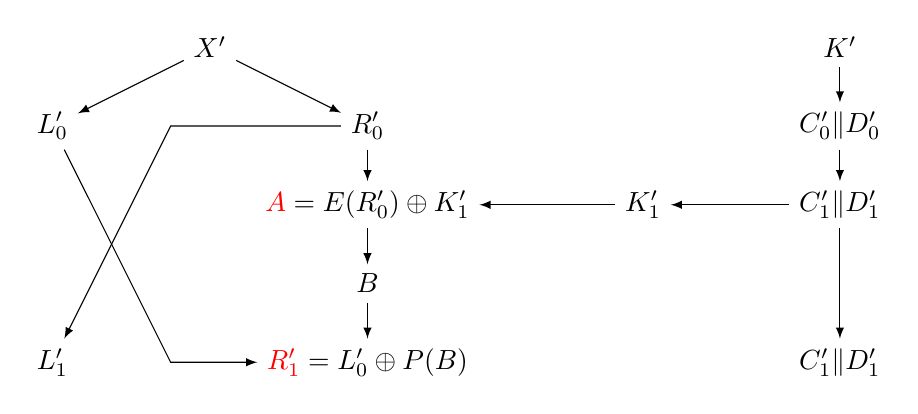
\begin{tikzpicture}

	% Left node definitions.
	\node (x_prime) at (2,4) {$X'$};
	\node   (l_not) at (0,3) {$L'_0$};
	\node   (r_not) at (4,3) {$R'_0$};
	\node       (a) at (4,2) {${\color{red}A} = E(R'_0) \oplus K'_1$};
	\node       (b) at (4,1) {$B$};
	\node   (l_one) at (0,0) {$L'_1$};
	\node   (r_one) at (4,0) {${\color{red}{R'_1}} = L'_0 \oplus P(B)$};

	% Right node definitions.
	\node    (k_prime) at  (10,4) {$K'$};
	\node  (pc1_of_kp) at  (10,3) {$C'_0 \Vert D'_0$};
	\node (left_shift) at  (10,2) {$C'_1 \Vert D'_1$};
	\node   (k1_prime) at (7.5,2) {$K'_1$};
	\node  (right_end) at  (10,0) {$C'_1 \Vert D'_1$};

	% Arrows.
	\draw[-latex]    (x_prime) -- (l_not);
	\draw[-latex]    (x_prime) -- (r_not);
	\draw[-latex]      (l_not) -- (1.5,0) -- (r_one);
	\draw[-latex]      (r_not) -- (1.5,3) -- (l_one);
	\draw[-latex]      (r_not) -- (a);
	\draw[-latex]          (a) -- (b);
	\draw[-latex]          (b) -- (r_one);
	\draw[-latex]    (k_prime) -- (pc1_of_kp);
	\draw[-latex]  (pc1_of_kp) -- (left_shift);
	\draw[-latex] (left_shift) -- (right_end);
	\draw[-latex] (left_shift) -- (k1_prime);
	\draw[-latex]   (k1_prime) -- (a);

\end{tikzpicture}
\end{document}